\documentclass{article}
\usepackage{doc,url,verbatim,fancyvrb}
\usepackage{pifont}
\usepackage[authoryear]{natbib}
\usepackage{gretl}
\usepackage{graphicx}
\usepackage[letterpaper,body={6.3in,9.15in},top=.8in,left=1.1in]{geometry}
\usepackage[pdftex,hyperfootnotes=false]{hyperref}

\usepackage[utf8]{inputenc}
\DeclareUnicodeCharacter{2212}{-}

\bibliographystyle{gretl}

\hypersetup{pdftitle={gretl + lpsolve},
            pdfauthor={Allin Cottrell},
            colorlinks=true,
            linkcolor=blue,
            urlcolor=red,
            citecolor=steel,
            bookmarks=true,
            bookmarksnumbered=true,
            plainpages=false
}

\begin{document}

\setlength{\parindent}{0pt}
\setlength{\parskip}{1ex}
\setcounter{secnumdepth}{1}

\newenvironment{funcdoc}
{\noindent\hrulefill\\[-10pt]}
{\medskip}

\newcommand{\argname}[1]{\textsl{#1}}

\title{gretl + lpsolve}
\author{Allin Cottrell}
\maketitle

\section{Introduction}
\label{sec:intro}

As of the 2021d release gretl offers support for \textsf{lpsolve}, an
open-source library for solving linear programming
problems.\footnote{For technical reasons this is not currently
  available in the 32-bit build of gretl for MS Windows. That may
  follow if we're able to resolve the problems we've encountered.}

While linear programming is not part of the standard econometrics
toolkit it surely falls under the rubric adopted in the founding of
the Econometric Society in 1930, namely ``to promote studies that aim
at a unification between the theoretical-quantitative and the
empirical-quantitative approach to economic problems.''\footnote{See
  \url{https://www.econometricsociety.org/society/about}.} And
some well known econometric studies have used linear programs as a
complement to estimation methodology---see for example
\cite{ferrier-lovell90}.

Section~\ref{sec:platforms} gives specifics per platform. Note that on
Linux you have to install the \textsf{lpsolve} package to activate
gretl's support.

\section{LP basics}
\label{sec:basics}

We're not going to say much here about Linear Programming in general,
or \textsf{lpsolve}'s \texttt{lp} file format in particular, since
there's plenty of good material at
\url{http://lpsolve.sourceforge.net/5.5/}. But we'll say enough to
establish notation for what follows, and give a brief overview of
\texttt{lp} format.

The basic expression of an LP problem in matrix form is
\begin{align*}
  \mbox{maximize} & \quad c'x \\
  \mbox{subject to} & \quad Ax \leq b \\
  & \quad x \geq 0
\end{align*}
where $x$ is an $n$-vector of variables and $c$ an $n$-vector of
coefficients, such that $c'x$ constitutes the objective function. In
the constraints on the variables $A$ is an $m\times n$ matrix of
coefficients and $b$ is an $m$-vector of upper limits. Note that in
\texttt{lpsolve} non-negativity constraints are implicit for all
elements of $x$; if you need to allow any negative values you must
contradict this assumption explicitly, as in ``\texttt{x1 >= -100;}''.

The native \textsf{lpsolve} file format---for which the standard
filename extension is ``\texttt{.lp}''---has the following
basic characteristics.
\begin{itemize}
\item Names of variables must start with a letter.
\item A comment can be opened with ``\texttt{/*}'' and closed with
  ``\texttt{*/}'', or ``\texttt{//}'' can be used for a single-line
  comment.
\item All statements are terminated with a semicolon.
\item The first statement should give the objective function, as a
  linear combination of variables (or a single variable).
\item Constraints are expressed as a linear combination of variables
  followed by an operator, followed by a constant.  The operator must
  be \texttt{<=}, \texttt{<}, \texttt{>=}, \texttt{>} or \texttt{=}.
  But note that \textsf{lpsolve} takes all inequality constraints to
  be real-valued, so \texttt{<=} and \texttt{<} are strictly
  equivalent, as are \texttt{>=} and \texttt{>}.
\item A trailing statement starting with the keyword \texttt{int} can
  be given to identify variables that are supposed to be integer
  valued, as in ``\texttt{int A, B;}''.
\end{itemize}

In \texttt{lp} format, each term of a linear combination must take the
form of a numerical constant (or an implicit 1) followed by the name
of a variable, as in ``\texttt{3 x}'' or just
``\texttt{3x}''. Multiplication is implicit (the symbol ``\texttt{*}''
is accepted but is not required or idiomatic). Parentheses are not
accepted. Here's an example constraint:
\begin{verbatim}
  A - 10 m1A - 20 m2A - 30 m3A = 0;
\end{verbatim}
See Section~\ref{sec:example} for a full example of usage.

\section{Implementation of lpsolve support}
\label{sec:implement}

There are two main ways of using \textsf{lpsolve} from within gretl.
\begin{itemize}
\item In the GUI program you can load or compose a linear program in
  the native format of \textsf{lpsolve}, send it for solution, and
  retrieve the results as native gretl objects.
\item Using either the GUI program or the command-line program
  \texttt{gretlcli}, you can formulate a linear program in various
  ways and call the \texttt{lpsolve()} function to obtain the solution
  in the form of a gretl bundle.
\end{itemize}

Some details follow.

\subsection{Via the GUI script editor}

A script in the default format of \textsf{lpsolve} can be loaded into
gretl by via the \textsf{File/Script files} menu or drag and drop.
Gretl expects a filename suffix of ``\texttt{.lp}'' for such files.
In the script editor you can modify the file if you wish, and execute
it via the toolbar or the \texttt{Ctrl+R} shortcut
(Figure~\ref{fig:kantor1}). The solution will be shown in an output
window. This window's toolbar will include a bundle button which pulls
down a menu allowing you to save the solution data
(Figure~\ref{fig:kantor2})

\begin{figure}[p]
  \centering
  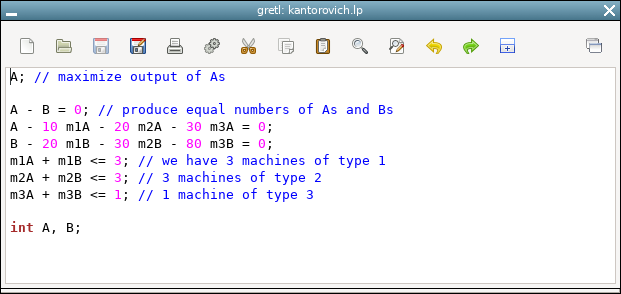
\includegraphics[scale=0.7]{figures/kantor-edit}
  \caption{Editing an \textsf{lpsolve} script. The execute icon is the
    sixth from the left.}
  \label{fig:kantor1}
\end{figure}

\begin{figure}[p]
  \centering
  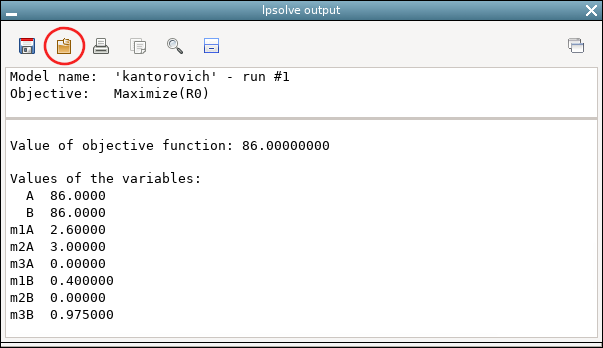
\includegraphics[scale=0.7]{figures/kantor-run}
  \caption{Partial output from an \textsf{lpsolve} run. The
    bundle-menu icon is the second from the left.}
  \label{fig:kantor2}
\end{figure}

\subsection{Via the \texttt{lpsolve} function}

The \texttt{lpsolve()} function has this signature:
\begin{verbatim}
  bundle lpsolve (const bundle specs)
\end{verbatim}

The input bundle, \texttt{specs}, must hold a specification of the
problem to be solved and may hold some optional elements.  The
problem specification itself may take any of these three forms:
\begin{itemize}
\item Under the key \texttt{lp\_filename}, the name of an \texttt{lp}
  file.
\item Under the key \texttt{lp\_buffer}, a multi-line string in
  \texttt{lp} format. Such a string can be composed using gretl's
  \texttt{sprintf} function and string concatenation. You can think of
  this as an \texttt{lp} file existing in memory rather than on disk.
\item Under the key \texttt{lp\_bundle}, a gretl bundle in which a
  linear program is represented by (primarily) a set of matrices. The
  requirements for such a bundle are set out in
  section~\ref{sec:lp-bundle} below.
\end{itemize}

\section{Top-level options}
\label{sec:gen-opts}

By ``top-level'' we mean that these options should be included
directly in the \texttt{specs} bundle passed to
\texttt{lpsolve()}. They apply regardless of the method by which the
linear program is specified.

\begin{itemize}
\item \texttt{minimize} (boolean, default 0): If this has a non-zero
  value the objective is minimized; by default it is maximized.  
\item \texttt{verbose} (boolean, default 0): If this has a non-zero
  value details of the solution process and results are
  printed. Otherwise \texttt{lpsolve()} runs silently unless the
  solver fails.
\item \texttt{sensitivity} (boolean, default 0): If this has a
  non-zero value additional output is provided as described in
  section~\ref{sec:retval}.
\item \texttt{model\_name} (string): If this is included it is shown
  when verbose output is produced.
\end{itemize}

\section{Contents of the return bundle}
\label{sec:retval}

Let $n$ and $m$ denote, respectively, the number of variables whose
values are to be optimized and the number of linear constraints.

The bundle returned by the \textsf{lpsolve} function includes the
following:
\begin{itemize}
\item \texttt{objective}: a scalar, the optimized value of the objective
  function.
\item \texttt{variable\_values}: an $n$-vector holding the optimized
  values of the variables.
\item \texttt{constraint\_values}: an $m$-vector holding the values of
  the constrained magnitudes at the solution.
\item \texttt{shadow\_prices}: an $m$-vector holding the Lagrange
  multipliers associated with the constraints.
\end{itemize}

In addition, if the \textsf{lpsolve} library version is 5.5.2.11 or
higher a scalar \texttt{accuracy} value is included. This gives the
accuracy with which the constraints are met; it is 0 at an exact
solution, larger values indicate approximation.

If the sensitivity option is activated the bundle contains an
additional $(n+m) \times 3$ matrix under the name
\texttt{sensitivity}. This holds all the dual variables along with the
lower and upper limits of their validity.

\section{Specifying a linear program via bundle}
\label{sec:lp-bundle}

A bundle given as \texttt{lp\_bundle} must have at least three
members, as follows.
\begin{enumerate}
\item \texttt{objective}: a row vector of length $n$ holding the
  coefficients on the variables in the linear objective
  function. Zeros must be inserted for variables that do not feature
  in the objective. If column names are attached to
  \texttt{objective} the variables are named accordingly in the
  printed output (if any) and the rows of \texttt{variable\_values}
  in the output bundle are named.
\item \texttt{constraints}: a matrix of dimension $m \times
  (n+1)$. Row $i$ holds the coefficient on each of the variables in
  constraint $i$ (again, with zeros inserted for any variables not
  referenced in the constraint), followed by the right-hand side
  value. If row names are attached to \texttt{constraints}, these
  names are used in the output.
\item \texttt{ctypes}: a specification of the types of the constraints
  (inequalities or equalities). It can take the form of an array of
  $m$ strings, each of which must be ``\texttt{<=}'', ``\texttt{>=}''
  or ``\texttt{=}'', or alternatively an $m$-vector in which these
  types are encoded as 1, 2 or 3, respectively.
\end{enumerate}

If you require that certain variables be integer-valued, you should
supply a fourth member of \texttt{lp\_bundle}: a matrix under the key
\texttt{intvars}. This is a vector holding the 1-based indices of the
variables in question.

\section{Platform specifics}
\label{sec:platforms}

In the gretl packages for 64-bit MS Windows and macOS, the
\textsf{lpsolve} library (as of this writing, version 5.5.2.11) is
included; no additional installation is required.

On Linux, however, it's easy to install the \textsf{lpsolve} library
via the package manager so we leave that up to the user. Here are the
commands that should be used on three popular Linux distributions:
\begin{center}
  \begin{tabular}{ll}
  Debian & \texttt{sudo apt-get install lp-solve} \\
  Fedora & \texttt{sudo dnf install lpsolve} \\
  Arch & \texttt{sudo pacman -S lpsolve}
\end{tabular}
\end{center}
After executing the relevant command it may be necessary to follow up
with
\begin{verbatim}
sudo ldconfig
\end{verbatim}
to ensure that the newly installed library can be found by gretl.

\section{Example}
\label{sec:example}

Consider L. V. Kantorovich's illustrative ``Example 1'' of 1939
(translated in \cite{kantorovich60}), one of the first linear programs
ever posed and solved. We require that two components of a finished
product, \texttt{A} and \texttt{B}, be produced in equal number and
that this number be maximized. The constraints take the form of the
numbers and capacities of machines of three different types that are
available for producing the components. The producer has three
machines of type 1, three of type 2, and one of type 3. The capacities
of these machines (maximum output per working day) are

\begin{center}
\begin{tabular}{cccc}
  & type 1 & type 2 & type 3 \\
  \texttt{A} & 10 & 20 & 30 \\
  \texttt{B} & 20 & 30 & 80 
\end{tabular}
\end{center}

To set up the LP problem we introduce the variables \texttt{m1A},
\texttt{m2A}, \texttt{m3A}, \texttt{m1B}, \texttt{m2B} and
\texttt{m3B}, where \texttt{m}$ij$ represents the type $i$
machine-days ($i=1,2,3$) devoted to production of component $j$ ($j=$
\texttt{A}, \texttt{B}).  The \textsf{lpsolve} script for this problem
was shown in Figure~\ref{fig:kantor1}; we reproduce it in
Listing~\ref{ls:kantor-lp} in case you want to copy and
paste. Listing~\ref{ls:kantor-inp} shows a simple script which passes
\texttt{kantorovich.lp} to the \textsf{lpsolve} library and returns a
bundle containing the results.

Listing~\ref{ls:kantor-bundle} shows how the same problem can be
specified by means of a gretl bundle rather than an \texttt{lp}
script. The bundle method may appear to be more cumbersome, but note
that it permits expression of the constraints in a structured manner,
using primary information such as (in the Kantorovich example) the
matrix \texttt{P} which holds the machine productivities.

Listing~\ref{ls:kantor-analysis} is a self-contained script for
execution by gretl which solves the problem (without printing
anything) and illustrates usage of information from the output
bundle. In the optimal solution to the Kantorovich problem 86
\texttt{A}s and \texttt{B}s are produced. The script shows the usage
rate of the three machine types: machines of type 1 and 2 are fully
employed but the type 3 machine has a little down-time, being employed
to 97.5\% of its capacity. The second piece of analysis shows that
machines of types 2 and 3 are fully specialized according to their
comparative advantage, while the type 1 machines produce both
\texttt{A}s and \texttt{B}s.


\begin{script}[htbp]
  \caption{Kantorovich's Example 1 as file \texttt{kantorovich.lp}}
  \label{ls:kantor-lp}
\begin{scode}
A; // maximize output of As

A - B = 0; // produce equal numbers of As and Bs
A - 10 m1A - 20 m2A - 30 m3A = 0;
B - 20 m1B - 30 m2B - 80 m3B = 0;
m1A + m1B <= 3; // we have 3 machines of type 1
m2A + m2B <= 3; // and 3 machines of type 2
m3A + m3B <= 1; // and 1 machine of type 3

int A, B; // require that A, B values be integers
\end{scode}
\end{script}

\begin{script}[htbp]
  \caption{Executing Kantorovich example in gretl}
  \label{ls:kantor-inp}
\begin{scode}
bundle b = _(lp_filename="kantorovich.lp", verbose=1)
bundle solution = lpsolve(b)
\end{scode}
\end{script}

\begin{script}[htbp]
  \caption{Kantorovich example specified via bundle}
  \label{ls:kantor-bundle}
\begin{scode}
set verbose off
string vnames = "A B m1A m2A m3A m1B m2B m3B"
nvars = 8

matrix Obj = zeros(1, nvars)
Obj[1] = 1
cnameset(Obj, vnames)
print Obj

# machine productivities (rows A B, cols m1 m2 m3)
matrix P = {10, 20, 30; 20, 30, 80}

matrix C = zeros(6, nvars+1)
C[1,1:2] = {1, -1}
C[2,1] = 1
C[2,3:5] = -P[1,]
C[3,2] = 1
C[3,6:8] = -P[2,]
C[4:6,3:9] = I(3) ~ I(3) ~ {3,3,1}'
string rnames = "A=B Asum Bsum nm1 nm2 nm3"
rnameset(C, rnames)
print C
strings Ops = defarray("=", "=", "=", "<=", "<=", "<=")

bundle lpb = _(objective=Obj, constraints=C, ctypes=Ops, intvars={1,2})
bundle specs = _(lp_bundle=lpb, model_name="kantorovich", verbose=1)
bundle ret = lpsolve(specs)
\end{scode}
\end{script}

\begin{script}[htbp]
  \caption{Use of information from the bundle returned by \texttt{lpsolve}}
  \label{ls:kantor-analysis}
Input:
\begin{scode}
set verbose off
bundle b = _(lp_filename="kantorovich.lp")
ret = lpsolve(b)
printf "\nTotal number of As and Bs produced: %d\n\n", ret.objective

matrix vv = ret.variable_values
matrix cv = ret.constraint_values

matrix u = cv[4:6]'
cnameset(u, "m1 m2 m3")
printf "Usage levels of machines:\n\n%8g\n", u

# machine productivities (rows: A, B)
matrix P = {10, 20, 30; 20, 30, 80}

# Outputs per machine type
matrix Q = zeros(2,3)
Q[1,] = vv[3:5]' .* P[1,]
Q[2,] = vv[6:8]' .* P[2,]
Q ~= sumr(Q)
cnameset(Q, "m1 m2 m3 sum")
rnameset(Q, "A B")
printf "Numbers of As and Bs produced per machine type:\n\n%6g\n", Q
\end{scode}
Output
\begin{scode}
Total number of As and Bs produced: 86

Usage levels of machines:

      m1      m2      m3
       3       3   0.975

Numbers of As and Bs produced per machine type:

      m1    m2    m3   sum
A     26    60     0    86
B      8     0    78    86
\end{scode}
\end{script}


\bibliography{gretl}

\end{document}
